\documentclass[12pt,]{article}
\usepackage{lmodern}
\usepackage{amssymb,amsmath}
\usepackage{ifxetex,ifluatex}
\usepackage{fixltx2e} % provides \textsubscript
\ifnum 0\ifxetex 1\fi\ifluatex 1\fi=0 % if pdftex
  \usepackage[T1]{fontenc}
  \usepackage[utf8]{inputenc}
\else % if luatex or xelatex
  \ifxetex
    \usepackage{mathspec}
  \else
    \usepackage{fontspec}
  \fi
  \defaultfontfeatures{Ligatures=TeX,Scale=MatchLowercase}
\fi
% use upquote if available, for straight quotes in verbatim environments
\IfFileExists{upquote.sty}{\usepackage{upquote}}{}
% use microtype if available
\IfFileExists{microtype.sty}{%
\usepackage{microtype}
\UseMicrotypeSet[protrusion]{basicmath} % disable protrusion for tt fonts
}{}
\usepackage[margin=1.0in]{geometry}
\usepackage{hyperref}
\hypersetup{unicode=true,
            pdftitle={Comparing Models of Subject-Clustered Single-Cell Data},
            pdfauthor={Audrey Hendricks*, PhD-Committee Chair and Advisor; Stephanie Santorico, PhD-Committee Member; Rhonda Bacher, PhD-Committee Member},
            pdfborder={0 0 0},
            breaklinks=true}
\urlstyle{same}  % don't use monospace font for urls
\usepackage{graphicx,grffile}
\makeatletter
\def\maxwidth{\ifdim\Gin@nat@width>\linewidth\linewidth\else\Gin@nat@width\fi}
\def\maxheight{\ifdim\Gin@nat@height>\textheight\textheight\else\Gin@nat@height\fi}
\makeatother
% Scale images if necessary, so that they will not overflow the page
% margins by default, and it is still possible to overwrite the defaults
% using explicit options in \includegraphics[width, height, ...]{}
\setkeys{Gin}{width=\maxwidth,height=\maxheight,keepaspectratio}
\IfFileExists{parskip.sty}{%
\usepackage{parskip}
}{% else
\setlength{\parindent}{0pt}
\setlength{\parskip}{6pt plus 2pt minus 1pt}
}
\setlength{\emergencystretch}{3em}  % prevent overfull lines
\providecommand{\tightlist}{%
  \setlength{\itemsep}{0pt}\setlength{\parskip}{0pt}}
\setcounter{secnumdepth}{5}
% Redefines (sub)paragraphs to behave more like sections
\ifx\paragraph\undefined\else
\let\oldparagraph\paragraph
\renewcommand{\paragraph}[1]{\oldparagraph{#1}\mbox{}}
\fi
\ifx\subparagraph\undefined\else
\let\oldsubparagraph\subparagraph
\renewcommand{\subparagraph}[1]{\oldsubparagraph{#1}\mbox{}}
\fi

%%% Use protect on footnotes to avoid problems with footnotes in titles
\let\rmarkdownfootnote\footnote%
\def\footnote{\protect\rmarkdownfootnote}

%%% Change title format to be more compact
\usepackage{titling}

% Create subtitle command for use in maketitle
\providecommand{\subtitle}[1]{
  \posttitle{
    \begin{center}\large#1\end{center}
    }
}

\setlength{\droptitle}{-2em}

  \title{Comparing Models of Subject-Clustered Single-Cell Data}
    \pretitle{\vspace{\droptitle}\centering\huge}
  \posttitle{\par}
  \subtitle{Lee Panter}
  \author{Audrey Hendricks*, PhD-Committee Chair and Advisor \\ Stephanie Santorico\footnote{The University of Colorado-Denver},
PhD-Committee Member \\ Rhonda Bacher\footnote{The University of Florida}, PhD-Committee Member}
    \preauthor{\centering\large\emph}
  \postauthor{\par}
    \date{}
    \predate{}\postdate{}
  
\usepackage{amsmath}
\usepackage{amsfonts}
\usepackage{amssymb}
\usepackage{enumitem}
\usepackage{graphicx}
\usepackage{array}
\usepackage{epsfig}
\usepackage{color}
\usepackage{multirow}
\usepackage{amsrefs}
\usepackage{placeins}
\usepackage[utf8]{inputenc}
\usepackage[english]{babel}
\usepackage{multicol}
\usepackage{comment}
\usepackage{multirow}
\usepackage{indentfirst}
\usepackage{listings}
\usepackage{setspace}
\usepackage{wrapfig}
\usepackage[right]{lineno}


\doublespacing
\setlength\parindent{15pt}
\setlength{\parskip}{3mm plus 1mm minus 1mm}

\lstset{frame=tb,
language=R,
aboveskip=3mm,
belowskip=3mm,
showstringspaces=false,
columns=flexible,
numbers=none,
keywordstyle=\color{blue},
numberstyle=\tiny\color{gray},
commentstyle=\color{dkgreen},
stringstyle=\color{mauve},
breaklines=true,
breakatwhitespace=true,
tabsize=3
}

\begin{document}
\maketitle

\hypertarget{abstract}{%
\section{Abstract}\label{abstract}}

\begin{onehalfspacing}

Single-Cell RNA sequencing data represents a revolutionary shift to approaches being used to decode the human transcriptome. Such data are becoming more prevalent and are gathered on ever-larger samples of individuals, enabling analysis of subject level relationships.  However, it is not always clear how to conduct this subject level analysis.  Current methods often do not account for nested study designs in which samples of hundreds, or thousands of cells are gathered from multiple individuals.  Therefore, there is a need to outline, analyze, and compare methods for estimating subject level relationships in single-cell RNA sequencing expression.  

Here, I compare five modeling strategies for detecting subject level associations using single-cell RNA sequencing expression: linear modeling, linear modeling with subjects modeled as fixed effects, linear mixed effects models with subjects modeled as random intercepts only or both random intercepts and random slopes, and generalized estimating equations.  I first present each method.  I then compare the regression estimates and standard errors for each method using real single-cell data from a Lupus Nephritis study of 27 subjects.  I hope that this paper presents insights into methods to analyze subject level associations from single-cell expression data.

\end{onehalfspacing}

\newpage

\setcounter{secnumdepth}{2}
\setcounter{tocdepth}{2}
\tableofcontents

\newpage

\hypertarget{introduction}{%
\section{Introduction}\label{introduction}}

Traditional methods of sequencing the human transcriptome involve
analyzing the combined genetic material of thousands or even millions of
cells. These so called ``bulk'' techniques provide information about the
average gene expression across the cell sample but often fail to capture
the underlying variability in expression profiles within the sample of
cells {[}1{]}.

Conversely, single-cell RNA sequencing (scRNA-seq) obtains measurements
of transcriptomic information specific to individual cells. Hundreds or
even thousands of RNA-sequencing profile measurements, each specific to
a single-cell, can be used to estimate expression variability across the
cells within the sample. This feature of single-cell data analysis is
suited for research applications that seek to identify rare cellular
subpopulations or characterize expressions that are differentially
expressed across conditions {[}2{]}. Additionally, technological
developments have made generating single-cell data more cost effective,
and easier to obtain on multiple sample-sources, most notably on
multiple individuals.

The utility of single-cell data, and the feasibility of single-cell data
measurements across multiple subjects motivates a need to compare
methods that can adequately model single-cell data while accounting for
the correlation of repeated measures within subjects (many single-cell
observations within each subject).

Here, I compare five methods for modeling scRNA-seq expression profiles
that account for within-subject correlation: linear modeling (LM),
linear modeling with subjects as fixed effects (LM-FE), linear mixed
effects models with subjects only as random intercepts (LMM-RI) or as
both random intercepts and random slopes (LMM-RS), and generalized
estimating equations (GEE). I first present the overall framework for
each method. Then I compare the results for each model using single-cell
data from a study of 27 Lupus Nephritis cases.

\hypertarget{description-of-data-set}{%
\section{Description of Data Set}\label{description-of-data-set}}

Throughout this paper references are made to the 2018 article entitled
``The immune cell landscape in kidneys with lupus nephritis patients'',
in which Arazi, Rao, Berthier, et al.~compare single-cell kidney tissue
sample data from 45 Lupus Nephritis subjects vs.~25 population controls
{[}3{]}. The kidney tissue samples were collected from ten clinical
sites across the United States, cryogenically frozen, then shipped to a
central processing facility. At the central processing facility, the
tissue samples were then thawed, and sorted into single-cell suspension
across 384-well plates using FlowJo 10.0.7, 11-color flow cytometry
{[}4{]}. Single-cell RNA sequencing was performed using a modified
CEL-Seq2 method {[}5{]} with \(\sim\) 1 million paired-end reads per
cell. The original experimental data may be accessed by visiting the
Immport repository with accession code SDY997.
\href{https://www.immport.org/shared/study/SDY997}{Immport-SDY997:
https://www.immport.org/shared/study/SDY997}

The original research conducted in Arazi, Rao, Berthier, et al,
concerned 70 subjects. A subset of 9,560 single-cell observations
originating from 27 subjects of the original data is used in the
analysis I conduct for this study. Markers of case/control status for
each subject are not present. However, for each single-cell observation
there are:

\begin{itemize}
\tightlist
\item
  Over \(3.8*10^{4}\) RNA sequencing measurements
\item
  23 Flow Cytometry measurements
\item
  10 meta data-variables (e.g.~subject of origin, cell type)
\end{itemize}

I implement a substantial quality control (QC) process to filter
observations that are inadequately representative of living,
single-cell, samples from an agglomerated Lupus Nephritis case/control
population. Inadequate (poor/low quality) observations are filtered out
if they are either: not a single-cell (i.e.~multiple, partial, or
missing cells), or cellular material that is insufficiently alive.
Details related to the QC filtering process are contained in
\textit{Appendix A-Data Quality Control}. After quality control filters
are imposed, 1110 observations originating from 15 subjects remain for
analysis.

I focus on two pairs of RNA sequencing variables for model comparisons.
I use the two outcome variables: \(MALAT1\) and \(FBLN1\) motivated by
previously established associations with human disease conditions
{[}6{]} {[}7{]}. I calculate pairwise correlations for each of the
chosen outcome variables, and I choose the Cluster of Differentiation
marker (see \textit{Appendix B-Variable Selections and Summaries} for
description) with the highest correlation to pair as a predictor to each
of the outcome variables. I perform a log-transformation on the
predictor and response of both variable pairings motivated by each
variable's right-skewed distribution.

I use the following transformed variable pairings to perform model
comparisons:

\begin{enumerate}
\def\labelenumi{\arabic{enumi}.}
\tightlist
\item
  \(log(MALAT1) \sim log(CD19)\)
\item
  \(log(FBLN1) \sim log(CD34)\)
\end{enumerate}

Further details related to variable selection and variable summaries are
contained in \textit{Appendix B-Variable Selections and Summaries}.

\hypertarget{model-descriptions}{%
\section{Model Descriptions}\label{model-descriptions}}

In the following sections a description is provided for each model using
the following notation for a subject level predictor-response pair:
\[\left(X_{ij},Y_{ij} \right)  \quad \text{for} \ \ i=1,\ldots,N \quad j=1,\ldots,n_{i} \]
where \(i=1,\ldots,N\) represents the observation's
\textit{subject of origination} (subject from which the measurement was
taken), and \(j=1,\ldots,n_{i}\) represents the measurement index taken
within subject \(i\) (the repeated measure index within each subject).

\newpage

\hypertarget{linear-model-lm}{%
\subsection{Linear Model (LM)}\label{linear-model-lm}}

The linear model can be written as:

\[Y_{ij}=\beta_{0} + \beta_{1} X_{ij} + \epsilon_{ij}\]

This model does not account for correlation structure in the data, and
instead assumes the observations are independent. Linear model parameter
estimates are for the population averages.

The error term, \(\epsilon_{ij}\), is assumed to be a normally
distributed random variable with mean zero and variance
\(\sigma_{\epsilon}^{2}\).

\hypertarget{linear-model-with-fixed-effect-lm-fe}{%
\subsection{Linear Model with Fixed-Effect
(LM-FE)}\label{linear-model-with-fixed-effect-lm-fe}}

Adding a subject specific fixed effect intercept term to the LM model
allows for the accounting of subject level effects by uniformly shifting
the mean of the fitted values specific to a subject. This model is
written as:

\[Y_{ij} = \beta_{0} + \beta_{1i}(subject_{j})+\beta_{2} X_{ij} + \epsilon_{ij}\]

where \[
\beta_{i}\left(subject_{j} \right)=
\begin{cases}
\beta_{i} & \mbox{if} \quad i=j \\
0 & \mbox{if} \quad i \neq j \\
\end{cases}
\quad \text{for} \quad i=2,\ldots,N\\
\]

This model adds \(N-1\) estimated parameters \(\hat{\beta}_{1i}\) which
represent the average deviation of each subject from the global
estimated mean Linear Model (LM).

\hypertarget{linear-mixed-effects-models}{%
\subsection{Linear Mixed Effects
Models}\label{linear-mixed-effects-models}}

Linear mixed effects models that incorporate multiple subjects using
random effects are the next methods outlined. Linear mixed effects
models do not require the assumption of independent observations.
Structures such as autoregressive, moving-average, or simply
unrestricted (unstructured) can be used to explicitly model
within-subject correlation. Additionally, random effects can be
incorperated and fit with covariance parameters that capture
between-subject effects.

\hypertarget{linear-mixed-effects-model-with-random-intercept-lmm-ri}{%
\subsubsection{Linear Mixed Effects Model with Random Intercept
(LMM-RI)}\label{linear-mixed-effects-model-with-random-intercept-lmm-ri}}

A linear mixed effects model with a random intercept controls for
subject-level correlations through the use of subject specific
variances. The LMM-RI model is written as:

\[Y_{ij} = \beta_{0} + \beta_{1} X_{ij} + b_{0i}\left(subject_{j}\right) + \epsilon_{ij}\]
where
\[b_{0i} \sim N\left(0, \sigma_{b}^{2} \right) \quad \epsilon_{ij} \sim N\left(0, \sigma_{\epsilon}^{2} \right)\]
\[\text{for} \quad i \in \left \{ 1,\ldots,N   \right \} \quad \text{and} \quad j \in \left \{ 1,\ldots,n_{i}   \right \}\]
it is assumed that \(b_{0i}\) and \(\epsilon_{ij}\) are independent.

\hypertarget{linear-mixed-effect-model-with-random-slope-lmm-rs}{%
\subsubsection{Linear Mixed Effect Model with Random Slope
(LMM-RS)}\label{linear-mixed-effect-model-with-random-slope-lmm-rs}}

A random slope linear mixed effects model differs from each of the
previously considered methods because it allows for distinct
relationships for each subject between the predictor and response
variables of interest. The LMM-RS model is written as:

\[Y_{ij} = \beta_{0} + \beta_{1} X_{ij} + b_{0i}\left(subject_{j}\right) + \left [ b_{1i}\left(subject_{j} \right) X_{ij}   \right ] + \epsilon_{ij}\]

where

\[\mathbf{b_{i}} = 
\begin{bmatrix}
b_{0i} \\
b_{1i}
\end{bmatrix} \sim 
N \left(\mathbf{0}, \mathbf{G} \right)\]

\[G=\begin{bmatrix}
\sigma_{b_{0}}^2 & \sigma_{b_{10}} \\
\sigma_{b_{10}} & \sigma_{b_{1}}^{2}\\
\end{bmatrix}\]

\[\epsilon_{ij} \sim N\left(\mathbf{0}, \sigma_{\epsilon}^{2}\mathbf{I}_{n_{i}} \right) \]
and it is still assumed that \(\mathbf{b}_{i}\) and \(\epsilon_{ij}\)
are independent for all \(j \in \left \{ 1, \ldots, n_{i} \right \}\)

\hypertarget{generalized-estimating-equations-gee}{%
\subsection{Generalized Estimating Equations
(GEE)}\label{generalized-estimating-equations-gee}}

The final modeling method considered is generalized estimating equations
(GEE). The GEE framework requires the specification of a systematic, and
random component. It also requires the specification of an assumed
covariance structure which approximates within-subject correlation, and
which the GEE algorithm iteratively re-fits estimated values. Each
iteration of the GEE algorithm incorperates information about all
subjects into successive estimates of parameters.

The components for the GEE model are:

\begin{itemize}
\tightlist
\item
  The random component

  \begin{itemize}
  \tightlist
  \item
    A probability distribution is assumed for the responses. The normal
    distribution is assumed here.
  \end{itemize}
\item
  The systematic component

  \begin{itemize}
  \tightlist
  \item
    The linear predictor, \(\eta_{ij}\), is a linear combination of the
    predictors. Here, there is only one predictor (\(X_{ij}\)), and the
    linear predictor used is:
    \[\eta_{ij} = \beta_{0} + \beta_{1} X_{ij}\]
  \end{itemize}
\item
  The link function

  \begin{itemize}
  \tightlist
  \item
    The link function \(g(\mu_{ij})=\mu_{ij}\) provides the relationship
    between the linear predictor and the expected outcome, i.e:
    \[E\left [Y_{ij} | X_{ij} \right ] = g(\mu_{ij}) = \mu_{ij}= \eta_{ij} = \beta_{0}+ \beta_{1} X_{ij}\]
  \end{itemize}
\item
  Working Covariance Structure

  \begin{itemize}
  \tightlist
  \item
    An independent working covariance structure is used here:
    \[\left [ Cov\left(Y_{ij}, Y_{ik}\right)\right ]_{jk}=
    \begin{cases}
    Var\left(Y_{ij}\right)  \quad &\mbox{if} \quad j=k \\
    0 \quad &\mbox{if} \quad j \neq k \\
    \end{cases}\]
    \[for \quad j,k \in \left \{  1, \ldots, n_{i}   \right \}\]
  \end{itemize}
\end{itemize}

Estimates for GEE parameters are calculated by solving an
\textit{estimating equation} using the Newton-Raphson iterative
root-finding algorithm. Detailed method descriptions, including
derivation and solving of the estimating equations can be found in
Fitzmaurice, Laird, and Ware {[}8{]}.

The GEE algorithm is robust to misspecification of the working
covariance structure. This means that initially incorrect specifications
of the working covariance matrix still converge to the appropriate
structure. This stability is due in-part to the fact that the method
estimates population average effects. This stability is also
attributable to the fact that GEE models the relationship between
response and covariate separate from an initially assumed, then
iteratively recalibrated correlation structure of the repeated measures
within grouping {[}9{]}.

\hypertarget{parameter-interpretations}{%
\subsection{Parameter Interpretations}\label{parameter-interpretations}}

The LM and GEE modeling methods are techniques used for obtaining
estimates of population averaged fixed effect slope parameters. These
parameter values are interpreted as contributing to the response of the
average subject (not representative of any single subject within the
sample). An example interpretation of this parameter is: \textbf{across
all subjects, a one-unit increase in the predictor (\(X_{ij}\)) is
associated with a \((\hat{\beta})\) unit change in the expected outcome
(\(Y_{ij}\)) of the average subject (assuming all other covariates are
held constant).}

\vspace{10pt}

The LMM-RI and LMM-RS modeling methods are techniques used for obtaining
estimates of subject specific fixed effect slope parameters. These
parameter values are interpreted as effects conitional on a specific
subject, contributing to the response of the specific subject. An
example interpretation of this parameter is: \textbf{after having
conditioned on and adjusted for the effects of a specific subject, a
one-unit increase in the predictor (\(X_{ij}\)) is associated with a
\((\hat{\beta})\) unit change in the expected outcome (\(Y_{ij}\)) of
that same subject (assuming all other covariates are held constant).}

\vspace{10pt}

Finally, the LM-FE method is a technique used for obtaining estimates of
population averaged fixed effect slope parameters adjusting for average
subject effects. These parameters are interpreted as contributing to the
response of the average subject after adjusting for a each subject's
average effect. An example interpretation of this parameter is:
\textbf{across all subjects, after having adjusted for the average
effect of each subject, a one-unit increase in the predictor
(\(X_{ij}\)) is associated with a \((\hat{\beta})\) unit change in the
expected outcome (\(Y_{ij}\)) of the average subject (assuming all other
covariates are held constant).}

\hypertarget{results}{%
\section{Results}\label{results}}

\hypertarget{parameter-value-comparisons}{%
\subsection{Parameter Value
Comparisons}\label{parameter-value-comparisons}}

A comparison of main effect slope coefficient, standard error and test
statistic (shown in \textbf{Tables (1) - (2)} below) across modeling
approaches within variable pairings indicates that estimates produced by
the LM and GEE methods are similar down to \(10^{-4}\). The LM-FE and
LMM-RI method estimates are also similar since estimates for each
parameter type (coefficient, standard error and test statistic) exhibit
magnitude and directional similarities in both variable pairings.

The LMM-RS estimates for the fixed effect slope parameter standard error
is the largest when compared to the corresponding estimates within
variable pairing as generated by other modeling methods. In contrast,
the standard error of the fixed effect slope parameter is smallest for
the LMM-RI model within variable pairings. The LM-FE model has a smaller
fixed effect slope standard error than either the LM or the GEE model
within both variable combinations.

The differences in test statistics of the fixed effect slope parameter
for each modeling method within each variable pairing are analogous to
the differences in slope coefficients previously noted. In particular,
test statistics have similar values between the LM and GEE models as
well as between the LM-FE and LMM-RI models. Test statistics calculated
for the LMM-RS model are the least similar to the other modeling
methods. The LMM-RS model averages test statistics that are 86\% larger
than the other models. This decreased similarity is also accompanied by
decreased parameter significance.

\vspace{5pt}

\small{
\begin{center}
\centering
\begin{tabular}{|m{0.15\textwidth}|m{0.275\textwidth}|c|c|c|c|}
\hline \noalign{\smallskip}
\center{Model \newline Designation} & \center{Model Description} & Estimate & Std. Error & Test Statistic & p-value \\
\hline
\hline
\center{LM} & \center{Linear Model} &  4.918e-2 &  1.455e-2  & 3.381 &  7.47e-4\\
\hline \noalign{\smallskip}
\center{LM-FE} & \center{Linear Model with  \newline Fixed-Effect Intercept} &  4.833e-2 &  1.381e-2 & 3.500 &  4.84e-4\\
\hline \noalign{\smallskip}
\center{LMM-RI} & \center{Linear Mixed Model with \newline Random Intercept} &  4.920e-2 &  1.374e-2 & 3.579  &  3.6e-4 \\
\hline \noalign{\smallskip}
\center{LMM-RS} & \center{Linear Mixed Model with \newline Random Slope }  & 5.938e-2 &  3.538e-2  & 1.678 &  1.19e-1 \\
\hline \noalign{\smallskip}
\center{GEE} & \center{Generalized Estimating Equations } & 4.918e-2 & 1.455e-2 & 3.381** & 7.47e-4 \\
\hline
\end{tabular}

\vspace{5pt}

\textbf{Table 1. $MALAT1 \sim CD19$ model estimates:} Fixed effect slope estimate, standard error, test statistic, and p-value for each model for the relationship between the predictor $CD19$ and the outcome $MALAT1$.  ** Approximate Wald-Z distribution.
\end{center}
}

\vspace{5pt}

\small{
\begin{center}
\centering
\begin{tabular}{|m{0.15\textwidth}|m{0.275\textwidth}|c|c|c|c|}
\hline \noalign{\smallskip}
\center{Model \newline Designation} & \center{Model Description} & Estimate & Std. Error & Test Statistic & p-value \\
\hline
\hline
\center{LM} & \center{Linear Model} &  7.884e-1 &  4.92e-2  & 4.002 & <2e-16\\
\hline \noalign{\smallskip}
\center{LM-FE} & \center{Linear Model with  \newline Fixed-Effect Intercept} &  1.31e-1 & 3.42e-2  & 3.818 & 1.42e-4 \\
\hline \noalign{\smallskip}
\center{LMM-RI} & \center{Linear Mixed Model with \newline Random Intercept} &  1.35e-1 & 3.42e-2  & 3.95 & 8.4e-5 \\
\hline \noalign{\smallskip}
\center{LMM-RS} & \center{Linear Mixed Model with \newline Random Slope }  & 1.705e-1  & 7.29e-2 & 2.34  & 6.7e-2 \\
\hline \noalign{\smallskip}
\center{GEE} & \center{Generalized Estimating Equations } & 7.884e-1 & 4.92e-2 & 4.002** & < 2e-16 \\
\hline
\end{tabular}

\vspace{5pt}

\textbf{Table 2. $FBLN1 \sim CD34$ model estimates:} Fixed effect slope estimate, standard error, test statistic, and p-value for each model for the relationship between the predictor $CD34$ and the outcome $FBLN1$.  ** Approximate Wald-Z distribution.
\end{center}
}

\newpage

Displayed in \textbf{tables (3)} - \textbf{(8)} below are percent change
in: parameter estimate, standard error, and test statistic for the
\(MALAT1 \sim CD19\) variable pairing in \textbf{tables (3)-(5)} and the
\(FBLN1 \sim CD34\) variable paring in \textbf{tables (6)-(8)}. Where
the percent change is defined as:
\[\text{Percent Change} \ [A]_{ij} = \left(\frac{A_{j}-A_{i}}{A_{i}}\right) * 100\]

\begin{center}
\begin{tabular}{|c||c|c|c|c|c|}
\hline
Model & LM & LM-FE & LMM-RI & LMM-RS & GEE \\
\hline
\hline
LM & 0 &  -1.7283 &  0.0407 & 20.7401 &  0.0000 \\
\hline
LM-FE & 1.7587 &  0 &  1.8001 & 22.8636  & 1.7587  \\      
\hline
LMM-RI & -0.0407 & -1.7683 &  0 & 20.6911 & -0.0407  \\
\hline
LMM-RS & -17.1775 & -18.6090 & -17.1438 & 0 & -17.1775 \\
\hline
GEE & 0.0000 & -1.7283  & 0.0407 & 20.7401  & 0 \\
\hline
\end{tabular}

\vspace{5pt}

\textbf{Table 3:} Main effect slope percent change matrix, $MALAT1 \sim CD19$ variable pairing
\end{center}

\vspace{20pt}

\begin{center}
\begin{tabular}{|c||c|c|c|c|c|c|}
\hline
Model & LM & LM-FE & LMM-RI & LMM-RS & GEE \\
\hline
\hline
LM & 0   & -5.0859  & -5.5670   & 143.1615  & 0.0000  \\
\hline
LM-FE & 5.3584   & 0   & -0.5069   & 156.1912  & 5.3584  \\     
\hline
LMM-RI & 5.8952   & 0.5095   & 0    & 157.4964  & 5.8952  \\
\hline
LMM-RS & -58.8751 & -60.9666 & -61.1645  & 0    & -58.8751  \\
\hline
GEE &  0.0000   & -5.0859  & -5.5670   & 143.1615  & 0        \\
\hline
\end{tabular}

\vspace{5pt}

\textbf{Table 4:} Main effect slope standard error percent change matrix, $MALAT1 \sim CD19$ variable pairing
\end{center}

\vspace{20pt}

\begin{center}
\begin{tabular}{|c||c|c|c|c|c|c|}
\hline
Model & LM & LM-FE & LMM-RI & LMM-RS & GEE \\
\hline
\hline
LM & 0  & 3.5197   & 5.8563    & -50.3697  & 0.0000 \\
\hline
LM-FE & -3.4000  & 0   & 2.2571    & -52.0571  & -3.4000 \\
\hline
LMM-RI & -5.5323  & -2.2073  & 0    & -53.1154  & -5.5323  \\
\hline
LM-RS & 101.4899 & 108.5816 & 113.2896  & 0    & 101.4899 \\
\hline
GEE & 0.0000  & 3.5197   & 5.8563    & -50.3697  & 0 \\
\hline
\end{tabular}

\vspace{5pt}

\textbf{Table 5:} Main effect slope test statistic percent change matrix, $MALAT1 \sim CD19$ variable pairing
\end{center}

\vspace{20pt}

\begin{center}
\begin{tabular}{|c||c|c|c|c|c|c|}
\hline
Model & LM & LM-FE & LMM-RI & LMM-RS & GEE \\
\hline
\hline
LM & 0   & -83.3841 & -82.8767  & -78.3739 & 0.0000  \\
\hline
LM-FE & 501.8321 & 0   & 3.0534    & 30.1527  & 501.8321 \\
\hline
LM-RI & 484.0000 & -2.9630  & 0    & 26.2963  & 484.0000  \\
\hline
LM-RS & 362.4047 & -23.1672 & -20.8211  & 0   & 362.4047  \\
\hline
GEE & 0.0000   & -83.3841 & -82.8767  & -78.3739 & 0  \\
\hline
\end{tabular}

\vspace{5pt}

\textbf{Table 6:} Main effect slope percent change matrix, $FBLN1 \sim CD34$ variable pairing
\end{center}

\vspace{20pt}

\begin{center}
\begin{tabular}{|c||c|c|c|c|c|c|}
\hline
Model & LM & LM-FE & LMM-RI & LMM-RS & GEE \\
\hline
\hline
LM & 0   & -30.4878 & -30.4878  & 48.1707   & 0.0000  \\
\hline
LM-FE & 43.8596  & 0   & 0.0000    & 113.1579  & 43.8596  \\
\hline
LM-RI & 43.8596  & 0.0000   & 0    & 113.1579  & 43.8596  \\
\hline
LM-RS & -32.5103 & -53.0864 & -53.0864  & 0    & -32.5103  \\
\hline
GEE &  0.0000   & -30.4878 & -30.4878  & 48.1707   & 0  \\
\hline
\end{tabular}

\vspace{5pt}

\textbf{Table 7:} Main effect slope standard error percent change matrix, $FBLN1 \sim CD34$ variable pairing
\end{center}

\vspace{20pt}

\begin{center}
\begin{tabular}{|c||c|c|c|c|c|c|}
\hline
Model & LM & LM-FE & LMM-RI & LMM-RS & GEE \\
\hline
\hline
LM & 0  & -4.5977  & -1.2994   & -41.5292  & 0.0000  \\
\hline
LM-FE & 4.8193  & 0   & 3.4573    & -38.7114  & 4.8193  \\
\hline
LM-RI & 1.3165  & -3.3418  & 0    & -40.7595  & 1.3165  \\
\hline
LM-RS & 71.0256 & 63.1624  & 68.8034   & 0    & 71.0256  \\
\hline
GEE & 0.0000  & -4.5977  & -1.2994   & -41.5292  & 0  \\
\hline
\end{tabular}

\vspace{5pt}

\textbf{Table 8:} Main effect slope test statistic percent change matrix, $FBLN1 \sim CD34$ variable pairing
\end{center}

\hypertarget{nested-model-comparisons}{%
\subsection{Nested Model Comparisons}\label{nested-model-comparisons}}

\begin{center}
\begin{tabular}{|c|c|c|c|c|c|c|c|}
\hline
Variable Pair & Model & Resid DF & RSS & DF & Sum of Squares & F-stat & P(>F) \\
\hline
\hline
\multirow{2}{*}{MALAT1-CD19} & LM & 1108 & 1167.76 & & & & \\
 & LM-FE & 1094 & 935.89 & 14 & 231.87 & 19.36 &  6.4776e-44 \\
\hline
\hline
\multirow{2}{*}{FBLN1-CD34} & LM & 1108 & 650.51 & & & & \\
 & LM-FE & 1094 & 214.92 & 14 & 435.59 & 158.38 &  2.8058e-251 \\
\hline
\hline
\end{tabular}

\vspace{5pt}

\textbf{Table 9:} ANOVA nested model comparison table for testing the inclusion of the subject specific fixed-effect intercept
\end{center}

(\textbf{Table 9}) above is a nested model comparison, the result of
which is an F-test statistic indicating that there sufficient evidence
to support the inclusion of the subject specific fixed-effect intercept
into the LM model.

\vspace{10pt}

\begin{center}
\begin{tabular}{|c|c|c|c|c|c|c|}
\hline
Variable Pair & Model & df & AIC & logLik & L.Ratio & p-value \\
\hline
\hline
\multirow{2}{*}{MALAT1-CD19} & LM & 3 & 3224.097 & -1609.048 &  & \\
 & LMM-RI & 4 & 3032.024 & -1512.012 & 194.0722 & 4.1068e-44  \\
\hline
\hline
\multirow{2}{*}{FBLN1-CD34} & LM & 3 & 2572.807 & -1283.403 &  & \\
 & LMM-RI & 4 & 1438.086 & -715.043 & 1136.72 & 3.4517e-249  \\
\hline
\hline
\end{tabular}

\vspace{5pt}

\textbf{Table 10:} ANOVA nested model comparison table for testing the inclusion of the subject specific random effect intercept
\end{center}

(\textbf{Table 10}) above is a nested model comparison, the result of
which is a likelihood ratio statistic indicating that there is
sufficient evidence to support the inclusion of the subject specific
random effect intercept into the LM model.

\vspace{15pt}

\begin{center}
\begin{tabular}{|c|c|c|c|c|c|c|}
\hline
Variable Pair & Model & df & AIC & logLik & L.Ratio & p-value \\
\hline
\hline
\multirow{2}{*}{MALAT1-CD19} & LMM-RI & 4 & 3032.024 & -1512.012 &  & \\
 & LMM-RS & 6 & 2993.820 & -1490.910 & 42.20503 & 6.8437e-10  \\
\hline
\hline
\multirow{2}{*}{FBLN1-CD34} & LMM-RI & 4 & 1438.086 & -715.043 &  & \\
 & LMM-RS & 6 & 1438.068 & -713.034 & 4.018095 & 0.1341  \\
\hline
\end{tabular}

\vspace{5pt}

\textbf{Table 11:} ANOVA nested model comparison table for testing the inclusion of the subject specific random effect slope
\end{center}

(\textbf{Table 11}) above is a nested model comparison, the result of
which is a likelihood ratio statistic idicating that there is sufficient
evidence to support the inclusion of the subject specific random effect
slope into the LMM-RI model for the \(MALAT1 \sim CD19\) variable
pairing. However, there is insufficient evidence to support the
inclusion of the subject specific random effect slope into the LMM-RI
model for the \(FBLN1 \sim CD34\) variable pairing.

\hypertarget{discussion}{%
\section{Discussion}\label{discussion}}

Here, I compared five modeling strategies for detecting subject level
associations in single-cell RNA sequencing data gathered over 27
subjects from a Lupus Nephritis study: linear modeling (LM), linear
modeling with subjects modeled as fixed effects (LM-FE), linear mixed
effects models with subjects modeled as only random intercepts (LMM-RI)
or random intercepts and random slopes (LMM-RS), and generalized
estimating equations (GEE). I find that population average models
(i.e.~LM and GEE) and the models which specify subject specific
intercept effects (i.e.~LM-FE and LMM-RI) tend to produce similar
results within the same description class (population average or subject
specific intercept effect models) but different results between model
classes. The highest standard errors are indicated in the LMM-RS model,
and the lowest standard errors in the LMM-RI model. LM-FE standard error
is also found to be smaller than both LM and GEE standard error values.
Nested model comparisons indicate that inclusion of subject specific
terms is advisable at all levels (fixed and random, intercept and slope)
with exception of the random slope in the \(FBLN1 \sim CD34\) variable
paring.

Each of the stated results is representative of some type of subject
level association within the single-cell RNA sequencing data I
investigated. The noted differences between estimates produced by
population average interpretation models LM/GEE and those produced by
the subject specific interpretation model LMM-RI is indicative of
subject specific, covariate independent associations not explicity
modeled by the overall population averaged model. Similarly, parameter
differences noted in comparisons with the LM-FE model estimates are
indicative of population average (having adjusted for average effect of
each subject), covariate independent associations not explicitly modeled
in the comparative model. Finally, an estimate that differs from those
generated by the LMM-RS method are idicative of a subject specific,
covariate dependent association not otherwise accounted for by the other
modeling technique.

In conjunction with the information gained through parameter estimate
comparisons, the nested model comparisons allow for further inference on
specific types of subject level associations. There is evidence for the
inclusion of all covariate terms into all models except for the random
slope into the LMM-RI model in the case of the \(FBLN1 \sim CD34\)
variable pairing. This coincides with intuition as differences were
noted between estimates generated by LMM/GEE compared to LM-FE/LMM-RI in
both variable pairings. The LMM-RS model was noted as having the largest
standard error, in addition to having the least similar estimate values.

The analysis I conducted in this paper has detected a variety of subject
level associations in single-cell RNA sequencing data using model
comparison techniques. I have detected subject level associations that
are related to: covariate dependency and parameter interpretation scope
(population average or subject specific). I have also demonstrated
method sensitivity. I used nested model comparison calculations to
reinforce detected associations when there was sufficient evidence to
suppot the underlying parameter's inclusion in a model, and I
deemphasized possible associations when insufficient evidence was
present.

The analyses performed here are subject to several drawbacks and
limitations. All the results are based on evidence obtained from just
two single-cell RNA sequencing variable pairings. In the future,
comparing the consistency of these models over all model pairs is
needed. Additionally, single-cell RNA sequencing data is heavily
influenced by protocol dependencies and measurement inconsistencies.
Quality control must be carefully considered and conducted prior to any
analysis.

The utility and promise of single-cell RNA sequencing data indicates
that such data will become more prevalent and will be extended to
multiple subject samples. I have presented an initial comparison of
methods for detecting subject-level associations in single-cell RNA
sequencing data sets.

\newpage

\hypertarget{appendix}{%
\section{Appendix}\label{appendix}}

\hypertarget{appendix-a-data-quality-control}{%
\subsection{Appendix A: Data Quality
Control}\label{appendix-a-data-quality-control}}

I use the Seurat Guided Clustering Tutorial {[}10{]} to perform quality
control (QC) of the initial data. This process quantifies the quality of
each single-cell observation in two numerical measures (based upon two
calculated variables, \(\mathbf{nFeature}\) and \(\mathbf{PerctMT}\)).
Threshold values of these variables are chosen and used to filter cells
(observations) not meeting the chosen criteria. The Seurat tutorial
provides methods of automated calculation and filtering implemented by
Arazi, Rao, Berthier, et al.~in {[}3{]}. Identical variable
calculations, with alternative threshold settings are independently
implemented for this study.

The quality control variables are conceptually defined as:

\begin{enumerate}
\def\labelenumi{\arabic{enumi}.}
\tightlist
\item
  \underline{$\mathbf{nFeature}$} is the number of unique genes detected
  to have a non-zero expression in each cell. This is used to identify
  cells with an abnormally low or high number of expressed genes. Low
  numbers may result from empty wells (zero content measurements) or
  broken (partial) cells, while high numbers may result from
  observations of more than one cell.
\item
  \underline{$\mathbf{PerctMT}$} is the percentage of reads that map to
  the mitochondrial genome. This is used to identify dead and/or broken
  cells as dead or dying cells will retain RNAs in mitochondria, but
  lose cytoplasmic RNA {[}2{]}.
\end{enumerate}

The pre-QC distribution of \(\mathbf{PerctMT}\) for each subject is
displayed in (\textbf{Figure A1}) below:

\newpage

\begin{figure}[!h]
\centering
        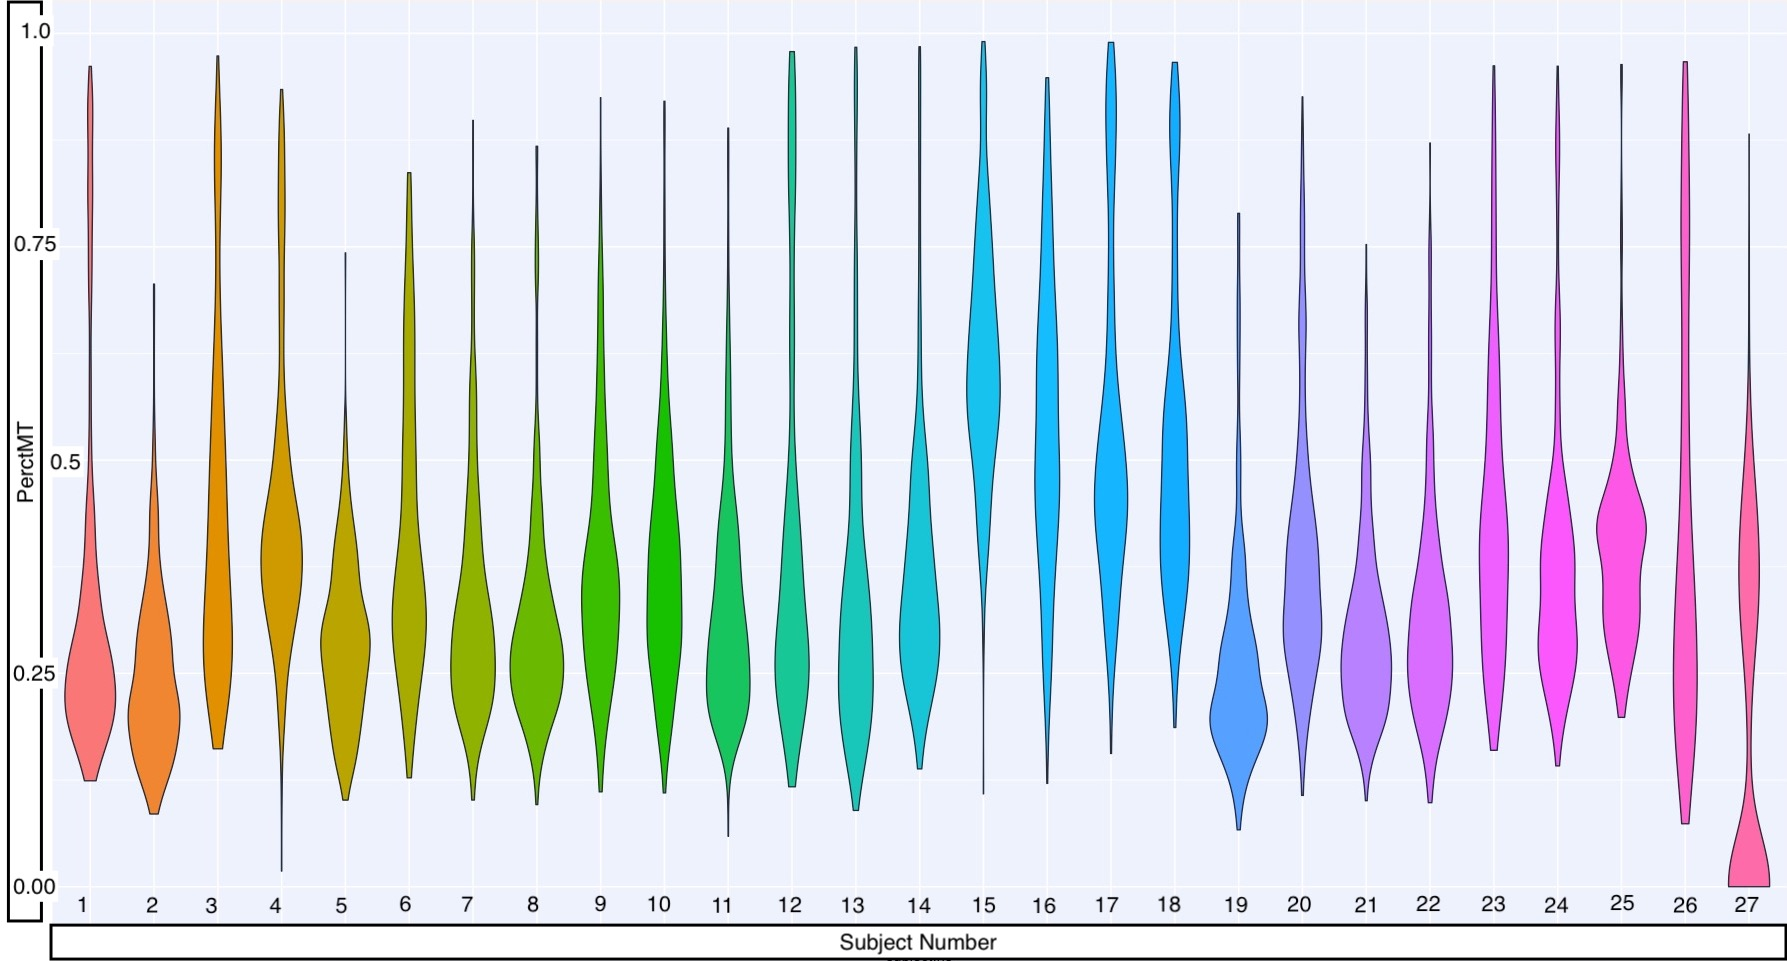
\includegraphics[width=0.75\textwidth]{fig1.jpeg}
\vspace{5pt}
\begin{center}
\textbf{Figure A1:} Pre-QC $\mathbf{PerctMT}$ Distribution for each subject
\end{center}
\end{figure}

The QC measure thresholds employed by Arazi, Rao, Berthier, et al.~in
{[}3{]} are:

\begin{enumerate}
\def\labelenumi{\arabic{enumi}.}
\tightlist
\item
  \(1,000 < \mathbf{nFeature} < 5,000\)
\item
  \(\mathbf{PerctMT} \leq 25 \%\)
\end{enumerate}

All observations for which the calculated values of
\(\mathbf{nFeature}\) and \(\mathbf{PerctMT}\) satisfied the
inequalities in (1) and (2) above were kept, and the others were
considered ``low-quality'' and removed. The resulting distribution of
the \(\mathbf{PerctMT}\) variable is displayed in (\textbf{Figure A2}):

\begin{figure}[!h]
\centering
        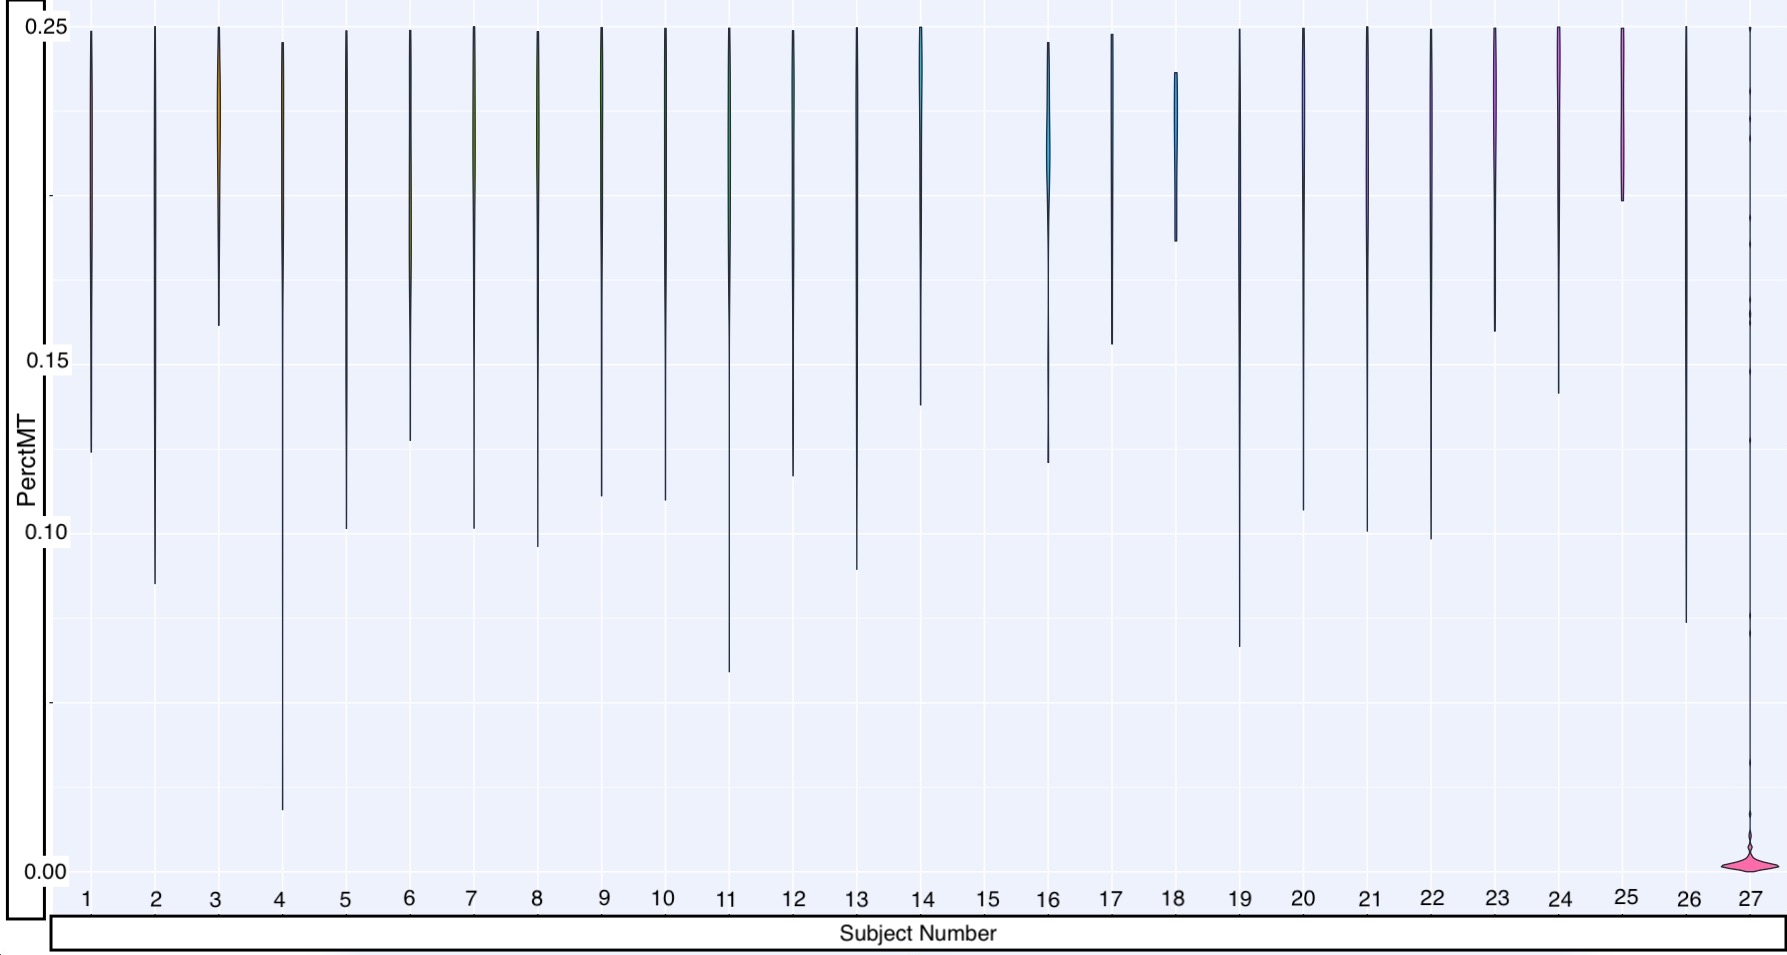
\includegraphics[width=0.7\textwidth]{fig2.jpeg}
\vspace{5pt}
\begin{center}
\textbf{Figure A2:} Post QC distribution of $\mathbf{PerctMT}$ with thresholds implemented by Arazi, Rao, Berthier, et al
\end{center}
\end{figure}

As 84\% of cells as removed with the filters chosen by Arazi et al, I
choose a more lenient threshold, removing observations with
\(\mathbf{PerctMT} \leq 60 \%\), in an effort to keep more cells.

An additional restriction of the data to only B-cells is made in an
effort to regularize the data sample (i.e.~homogenize feature
expression). The resulting distribution of \(\mathbf{PerctMT}\) is
displayed in (\textbf{Figure A3}) after filtering.

\begin{figure}[!h]
\centering
        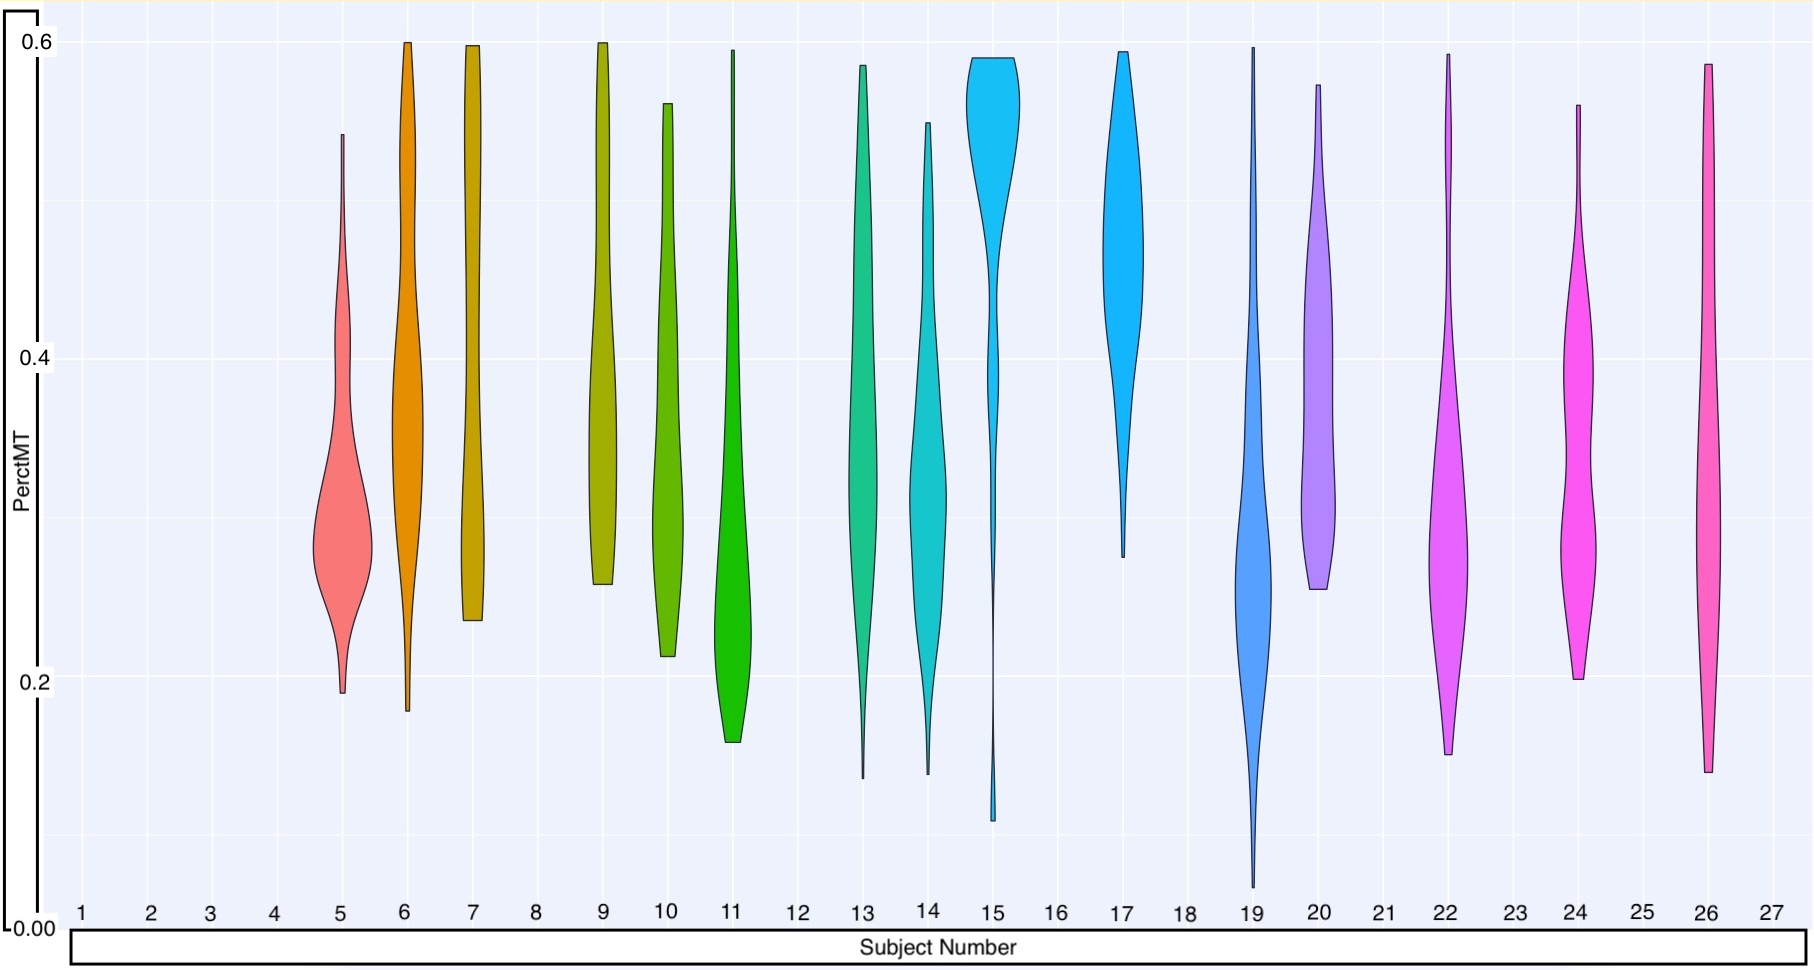
\includegraphics[width=0.75\textwidth]{fig3.jpeg}
\vspace{5pt}
\begin{center}
\textbf{Figure A3:} Post QC distribution of $\mathbf{PerctMT}$ with thresholds implemented in this paper
\end{center}
\end{figure}

The distribution of observations for each subject Pre/Post QC (with
updated \newline \(\mathbf{PerctMT} \leq 60 \%\) threshold value) is
shown numerically in (\textbf{Table A1}):

\vspace{5pt}
\begin{center}
\begin{tabular}{|c||c|c|c|c|c|c|c|c|c|}
\hline
\textbf{Subject Number} & \textbf{1} & \textbf{2} & \textbf{3} & \textbf{4} & \textbf{5} & \textbf{6} & \textbf{7} & \textbf{8} & \textbf{9}  \\
\hline
\hline
\textbf{NO of Obs Before QC} & 375 & 375 & 364 & 381 & 340 & 383 & 383 & 356 & 372 \\
\hline
\textbf{NO of Obs After QC} & 0 & 0 & 0 & 0 & 58 & 86 & 32 & 0 & 31 \\
\hline
\hline
\textbf{Subject Number} & \textbf{10} & \textbf{11} & \textbf{12} & \textbf{13} & \textbf{14} & \textbf{15} & \textbf{16} & \textbf{17} & \textbf{18}  \\
\hline
\hline
\textbf{NO of Obs Before QC}  & 327 & 311 & 379 & 375 & 345 & 371 & 381 & 381 & 377 \\
\hline
\textbf{NO of Obs After QC} & 21 & 107 & 0 & 107 & 100 & 25 & 0 & 122 & 0 \\
\hline
\hline
\textbf{Subject Number} & \textbf{19} & \textbf{20} & \textbf{21} & \textbf{22} & \textbf{23} & \textbf{24} & \textbf{25} & \textbf{26} & \textbf{27}  \\
\hline
\hline
\textbf{NO of Obs Before QC} & 380 & 381 & 380 & 333 & 333 & 239 & 218 & 378 & 342 \\
\hline
\textbf{NO of Obs After QC} & 127 & 75 & 0 & 87 & 0 & 79 & 0 & 53 & 0 \\
\hline
\end{tabular}
\end{center}
\vspace{5pt}

\begin{center}
\textbf{Table A1:} Observation counts per-subject Pre/Post QC with updated $\mathbf{PerctMT} \leq 60 \%$ threshold value.
\end{center}

\vspace{5pt}

\begin{center}
\begin{tabular}{|c|c|c|c|c|c|}
\hline
MIN & 1st Q & Median & Mean & 3rd Q & MAX \\
\hline
21 & 42.5 & 79 & 74.0 & 103.5 & 127 \\
\hline
\end{tabular}

\vspace{5pt}

\textbf{Table A2:} observation count per-subject summary statistics Post QC with updated $\mathbf{PerctMT} \leq 60 \%$ threshold value
\end{center}

\hypertarget{appendix-b-variable-selection-and-summaries}{%
\subsection{Appendix B: Variable Selection and
Summaries}\label{appendix-b-variable-selection-and-summaries}}

I select two pairs of variables from the 38,354 genetic markers in the
Lupus Data to compare across the five modeling methods. The variables I
choose have higher values of correlation than arbitrary variable
pairings as indicated by a high Pearson Correlation Coefficient (both
selected pairings are within the top 10\% of highest Pearson Correlation
Coefficients of all possible pairings), and have previously been
associated with human diseases or conditions (e.g.~cancer treatment
research in the case of MALAT1 {[}6{]}-used as the first outcome, or
observed limb malformations in the case of FBLN1 {[}7{]}-used as the
second outcome). I also attempt to assign predictor-pairings of
interest. The CD19 marker (the predictor paired with MALAT1) is a
transmembrane protein encoded by the CD19 gene. The FlowJo cytometry
measurements contain CD19 protein readings, so the relationship between
CD19 as a predictor and the outcome of interest (MALAT1) can be modeled
using proteomic or transcriptomics data. CD34, the predictor which I
link with FBLN1 is also a transmembrane protein encoded by a gene, and
similarly interesting.

Without undergoing the process of expression normalization, single-cell
RNA sequencing data is represented as non-negative integer count values.
Higher counts correspond to higher detection frequencies and these
detection frequencies can be interpreted as a quantification of the
magnitude of expression for a transcriptomic marker (e.g CD19, CD34,
MALAT1, FBLN1).

I provide numerical summaries of the four selected variables in
\textbf{Tables (B3) - (B6)}. Each describes selected variable summary
statistics (minimum, maximum, average, and median) for the positive
observational count subjects in (\textbf{Table A1}).

Measurements of scRNA-seq data are specific to precise transcriptomic
targets. This means that single-cell expression profiles (a single
observation) can be limited to a small transcriptomic scope. So while
the agglomerated scope of gene expression across a sample is the same as
(or broader than) a traditional bulk experiment, individual observations
have a biologically inflated zero-component. There are also
\textit{technical} zero-inflation components that are associated with
protocol variations, and measurement error. Together, these factors
contribute to right-skewed variable distributions (\textbf{Figure B1})

\begin{figure}[h!]
\centering
        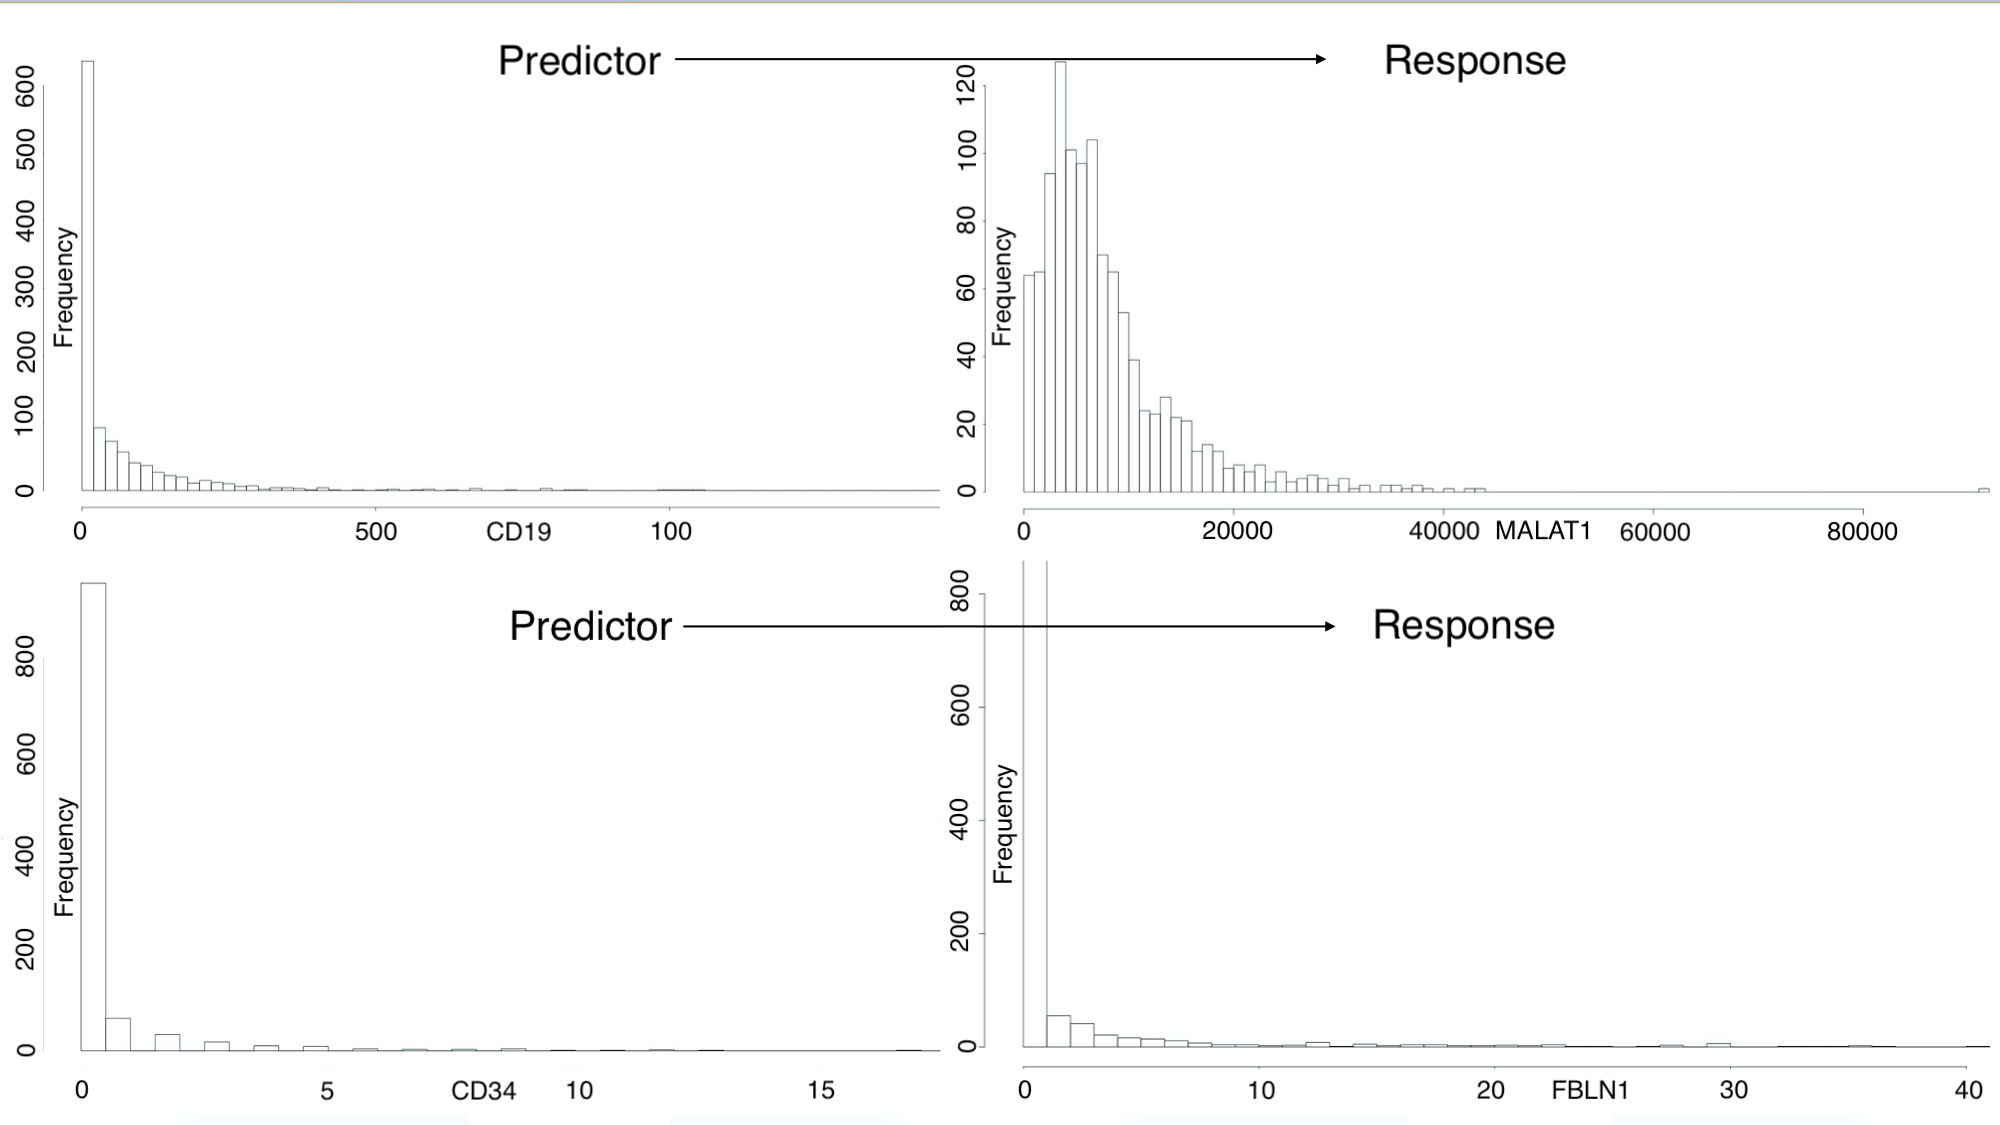
\includegraphics[width=0.85\textwidth]{Untranslated.jpg}
\end{figure}

\vspace{5pt}

\begin{center}
\textbf{Figure B1:} Predictor-Response pairing variable distributions
\end{center}

The MALAT1 variable has a large minimum outcome compared to the other
variables, so I translate all the values of this variable
\textit{negatively} by the minimum value. \[min(\text{MALAT1})=67\] This
gives a minimum expression value of zero, which coincides with intuition
as well as the minimum value of the other variables under investigation.

The modeling methodologies I employ motivate a log-transformation in an
attempt to achieve approximate normality, especially for the outcome
variable's distribution. I perform the ``log plus +1'' transformation on
all variables (predictor and outcome):
\[X \mapsto \log \left(X+1\right) \] The resulting distributions are
shown in (\textbf{Figure B2})

\begin{figure}[h!]
\centering
        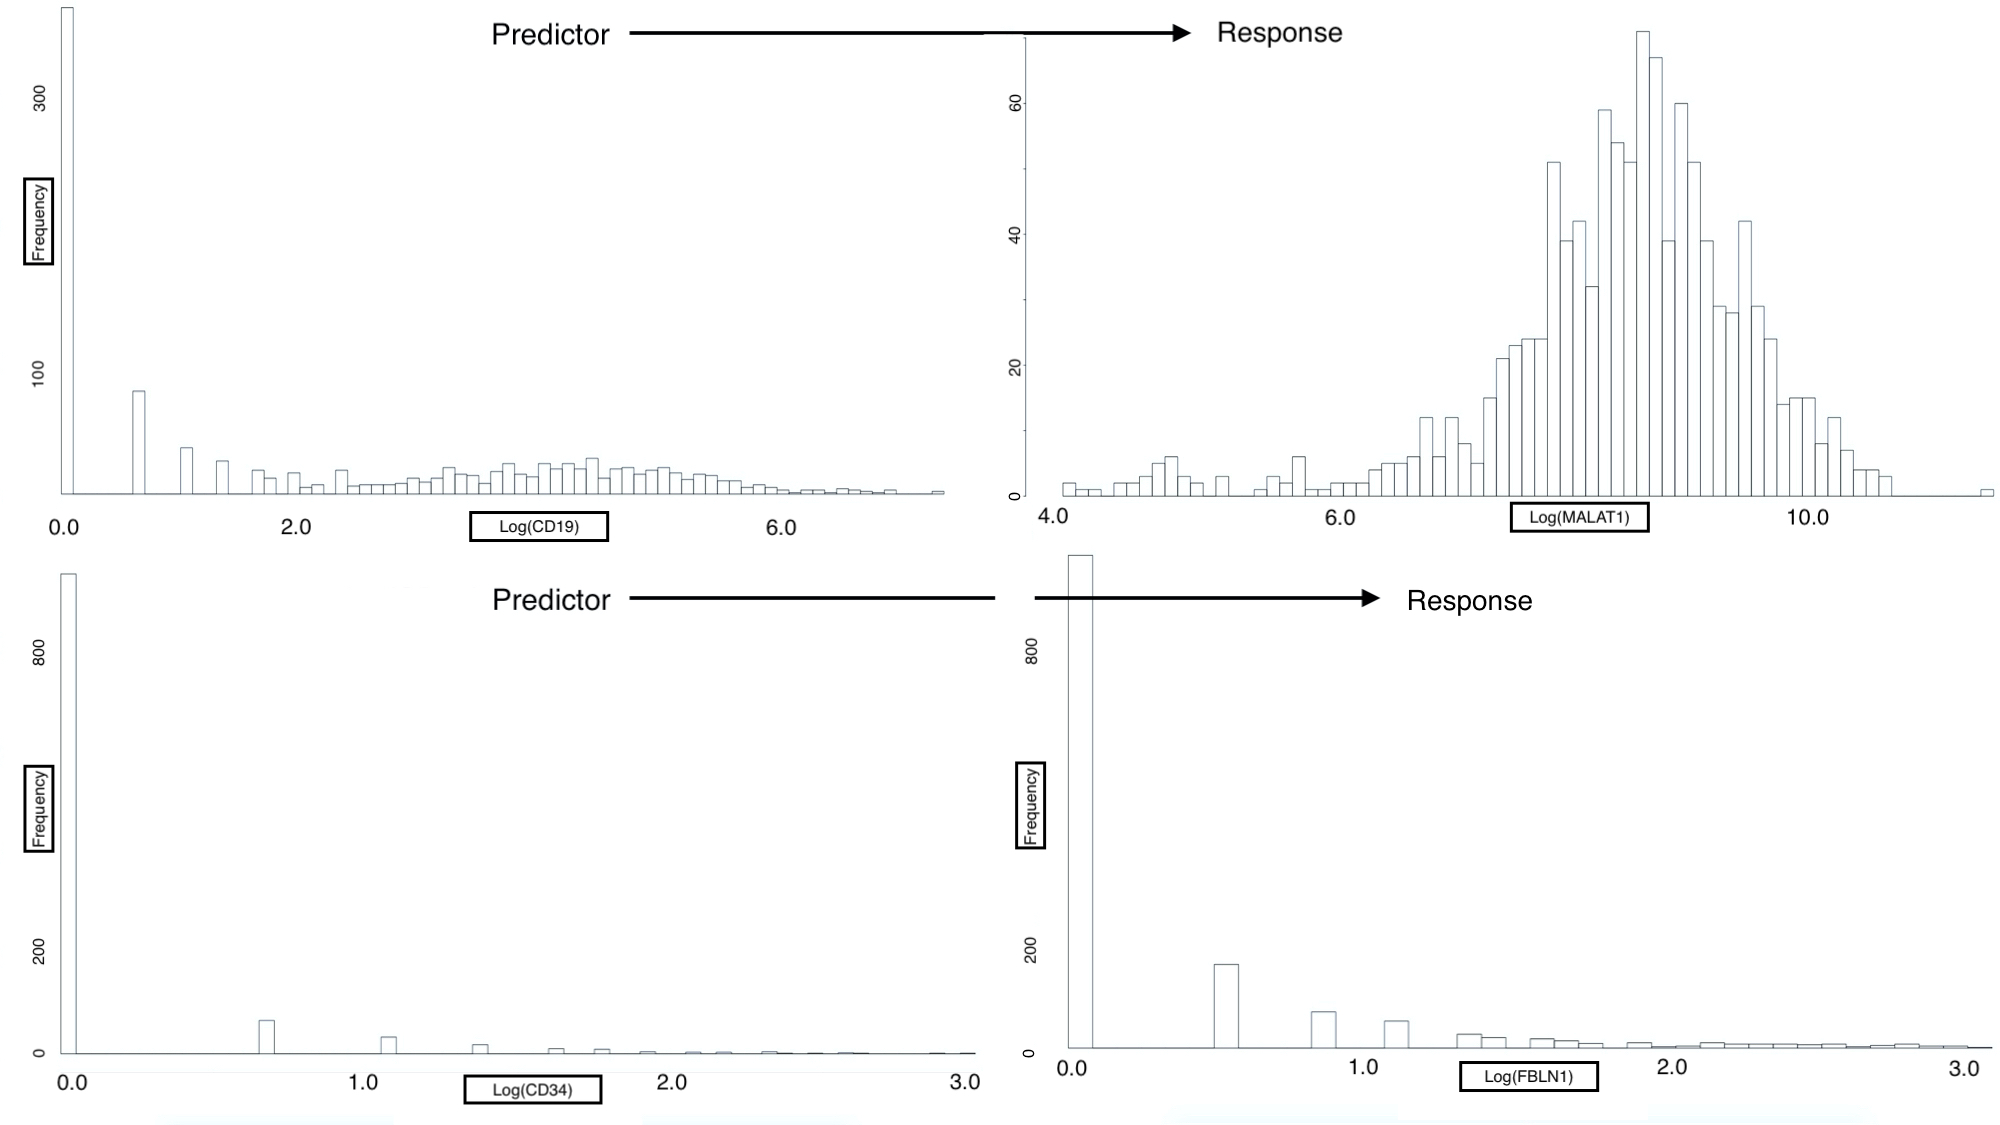
\includegraphics[width=0.85\textwidth]{Transformed.jpg}
\end{figure}
\vspace{5pt}
\begin{center}
\textbf{Figure B2:} Predictor-Response variable pairings, post-transformation distributions
\end{center}

The log-transformed response of MALAT1 is approximately normally
distributed; however, the log-transformed response FBLN1 is not
inherently better than the un-transformed response.

Regardless, each outcome is modeled under the assumption that:
compensating for observational correlation will sufficiently account for
non-normality of the responses. It may be the case that additional
transformations and/or alternative modeling techniques may be needed to
improve model error distributions. However, for the purpose of comparing
the previously mentioned models on subject-correlated single-cell data,
I proceed with this assumption and I verify residual homoscedasticity,
normality and independence using fitted vs residual plots and
quantile-quantile plots.

\hypertarget{variable-summary-tables}{%
\subsubsection{Variable Summary Tables}\label{variable-summary-tables}}

\textbf{Tables (B3) - (B6)} are summary tables for the variables chosen
in this analysis. The data in each table pertains to a subject that had
non-zero post quality control observation counts (i.e.~the subject had
data that past quality control filters). All values displayed are
calculated on post-qc data.

\newpage

\begin{center}

\textbf{\large{Table B3: CD19 Summaries}}

\begin{scriptsize}
\begin{tabular}{|c|c|c|c|c|}
\hline 
Subject Number & Minimum & Maximum & Average & Median \\ 
\hline
\hline
5 &  0 & 678 & 36.6724 & 0.0 \\ 
\hline  
6 &  0 & 299 & 36.6860 & 7.5 \\ 
\hline  
7 &  0 & 10 & 2.1250 & 1.0 \\ 
\hline  
9 &  0 & 1052 & 89.4194 & 3.0 \\ 
\hline  
10 & 0 & 158 & 37.5714 & 2.0 \\ 
\hline   
11 & 0 & 339 & 28.3178 & 1.0 \\ 
\hline   
13 & 0 & 629 & 56.0841 & 18.0 \\ 
\hline   
14 & 0 & 251 & 42.2600 & 19.0 \\ 
\hline   
15 & 0 & 148 & 26.6000 & 0.0 \\ 
\hline   
17 & 0 & 982 & 112.3770 & 16.0 \\ 
\hline   
19 & 0 & 665 & 59.3386 & 5.0 \\ 
\hline   
20 & 0 & 287 & 40.1200 & 23.0 \\ 
\hline   
22 & 0 & 380 & 43.4483 & 1.0 \\ 
\hline   
24 & 0 & 282 & 55.0127 & 27.0 \\ 
\hline  
26 & 0 & 1624 & 268.4151 & 110.0 \\  
\hline
\end{tabular}

\vspace{5pt}

\textbf{Table B3:} Predictor $CD19$ variable summaries ($CD19 \sim MALAT1$)
\end{scriptsize}
\end{center}

\begin{center}

\textbf{\large{Table B4: MALAT1 Summaries}}

\begin{scriptsize}
\begin{tabular}{|c|c|c|c|c|}
\hline 
Subject Number & Minimum & Maximum & Average & Median \\ 
\hline
\hline
5  & 67 & 40812 & 10206.3621 & 9195.0 \\ 
\hline 
6  & 757 & 30774 & 11568.2791 & 11689.0 \\ 
\hline 
7  & 441 & 17916 & 6868 & 4039.5 \\ 
\hline 
9  & 311 & 18239 & 5703.9355 & 5983.0 \\ 
\hline 
10 & 1875 & 17160 & 6638.5714 & 6190.0 \\ 
\hline
11 & 349 & 34082 & 9716.0280 & 8826.0 \\ 
\hline 
13 & 99 & 25572 & 5867.9439 & 4895.0 \\ 
\hline 
14 & 355 & 15740 & 6154.1500 & 5720.5 \\ 
\hline 
15 & 157 & 11923 & 3839.0800 & 3467.0 \\ 
\hline 
17 & 337 & 8342 & 2960.2541 & 2692.0 \\ 
\hline 
19 & 227 & 91961 & 13959.9843 & 10125.0 \\ 
\hline 
20 & 379 & 21736 & 7301.4133 & 6417.0 \\ 
\hline 
22 & 161 & 28429 & 6881.7471 & 5068.0 \\ 
\hline 
24 & 240 & 42792 & 6248.8228 & 5955.0 \\ 
\hline 
26 & 1114 & 32426 & 8463.1698 & 6426.0 \\ 
\hline  
\end{tabular}

\vspace{5pt}

\textbf{Table B4:} Response $MALAT1$ variable summaries ($CD19 \sim MALAT1$)

\end{scriptsize}
\end{center}

\newpage

\begin{center}
\begin{scriptsize}
\textbf{\large{Table B5: CD34 Summaries}}


\begin{tabular}{|c|c|c|c|c|}
\hline 
Subject Number & Minimum & Maximum & Average & Median \\ 
\hline
\hline
5  & 0 & 19 & 3.0517 & 1 \\ 
\hline 
6  & 0 & 0 & 0 & 0 \\ 
\hline 
7  & 0 & 0 & 2 & 1 \\ 
\hline 
9  & 0 & 6 & 0.4516 & 0 \\ 
\hline 
10 & 0 & 5 & 0.6667 & 0 \\ 
\hline 
11 & 0 & 7 & 1.2056 & 1 \\ 
\hline 
13 & 0 & 0 & 0 & 0 \\ 
\hline 
14 & 0 & 1 & 0.4000 & 0 \\ 
\hline 
15 & 0 & 0 & 0 & 0 \\ 
\hline 
17 & 0 & 0 & 0 & 0 \\ 
\hline 
19 & 0 & 0 & 0 & 0 \\ 
\hline 
20 & 0 & 2 & 0.1867 & 0 \\ 
\hline 
22 & 0 & 4 & 0.3563 & 0 \\ 
\hline 
24 & 0 & 5 & 0.2911 & 0 \\ 
\hline 
26 & 0 & 0 & 0 & 0 \\  
\hline
\end{tabular}

\vspace{5pt}

\textbf{Table B5:} Predictor $CD34$ variable summaries ($CD34 \sim FBLN1$)

\end{scriptsize}
\end{center}

\begin{center}
\begin{scriptsize}

\textbf{\large{Table B6:FBLN1 Summaries}}


\begin{tabular}{|c|c|c|c|c|}
\hline 
Subject Number & Minimum & Maximum & Average & Median \\ 
\hline
\hline
5  & 3 & 41 & 19.3448 & 18 \\ 
\hline 
6  & 0 & 0 & 0 & 0 \\ 
\hline 
7  & 0 & 16 & 4.2500 & 3 \\ 
\hline 
9  & 0 & 8 & 1.8710 & 1 \\ 
\hline 
10 & 0 & 30 & 11.9524 & 10 \\ 
\hline 
11 & 0 & 8 & 1.5140 & 1 \\ 
\hline 
13 & 0 & 1 & 0.0093 & 0 \\ 
\hline 
14 & 0 & 5 & 0.5700 & 0 \\ 
\hline 
15 & 0 & 1 & 0.0400 & 0 \\ 
\hline 
17 & 0 & 3 & 0.0246 & 0 \\ 
\hline 
19 & 0 & 2 & 0.0157 & 0 \\ 
\hline 
20 & 0 & 9 & 2.5867 & 2 \\ 
\hline 
22 & 0 & 11 & 0.9885 & 0 \\ 
\hline 
24 & 0 & 4 & 0.4557 & 0 \\ 
\hline 
26 & 0 & 0 & 0 & 0 \\ 
\hline
\end{tabular}

\vspace{5pt}

\textbf{Table B6:}: Response $FBLN1$ variable summaries ($CD34 \sim FBLN1$)

\end{scriptsize}
\end{center}

\newpage

\hypertarget{code-and-data}{%
\section{Code and Data}\label{code-and-data}}

All code for the above analysis was written and evaluated in RStudio
Version 1.2.1335, and is available for download at the following GitHub
repository:

\url{https://github.com/leepanter/MSproject_RBC.git}

Additionally, a link to all necessarry and referrence data files
(including original data) are contained in the following Google Drive:

\url{https://drive.google.com/open?id=1gjHaMJG0Y_kPYWj5bIE4gRJU5z9R2Wqb}

\hypertarget{references}{%
\section{References}\label{references}}

\bibliography{Bib_AccRefSheet}

\hypertarget{refs}{}
\leavevmode\hypertarget{ref-macaulay2014single}{}%
1. Macaulay IC, Voet T (2014) Single cell genomics: Advances and future
perspectives. \emph{PLoS genetics} 10: e1004126.

\leavevmode\hypertarget{ref-bacher2016design}{}%
2. Bacher R, Kendziorski C (2016) Design and computational analysis of
single-cell rna-sequencing experiments. \emph{Genome biology} 17: 63.

\leavevmode\hypertarget{ref-arazi2018immune}{}%
3. Arazi A, Rao DA, Berthier CC, et al. (2018) The immune cell landscape
in kidneys of lupus nephritis patients. \emph{bioRxiv} 363051.

\leavevmode\hypertarget{ref-flowjov10}{}%
4. FlowJo X V10. 0.7 r2 flowjo. \emph{LLC https://www flowjo com}.

\leavevmode\hypertarget{ref-hashimshony2016cel}{}%
5. Hashimshony T, Senderovich N, Avital G, et al. (2016) CEL-seq2:
Sensitive highly-multiplexed single-cell rna-seq. \emph{Genome biology}
17: 77.

\leavevmode\hypertarget{ref-gutschner2013malat1}{}%
6. Gutschner T, Hämmerle M, Diederichs S (2013) MALAT1---a paradigm for
long noncoding rna function in cancer. \emph{Journal of molecular
medicine} 91: 791--801.

\leavevmode\hypertarget{ref-debeer2002fibulin}{}%
7. Debeer P, Schoenmakers E, Twal W, et al. (2002) The fibulin-1 gene
(fbln1) is disrupted in at (12; 22) associated with a complex type of
synpolydactyly. \emph{Journal of medical genetics} 39: 98--104.

\leavevmode\hypertarget{ref-fitzmaurice2012applied}{}%
8. Fitzmaurice GM, Laird NM, Ware JH (2012) Applied longitudinal
analysis, John Wiley \& Sons.

\leavevmode\hypertarget{ref-odueyungbo2008comparison}{}%
9. Odueyungbo A, Browne D, Akhtar-Danesh N, et al. (2008) Comparison of
generalized estimating equations and quadratic inference functions using
data from the national longitudinal survey of children and youth (nlscy)
database. \emph{BMC medical research methodology} 8: 28.

\leavevmode\hypertarget{ref-satija2018seurat}{}%
10. Satija R, others (2018) Seurat: Guided clustering tutorial.
\emph{Satija Lab http://satijalab org/seurat/pbmc3k\_tutorial html}.


\end{document}
